\documentclass{my_paper}
\usepackage{ctex}
\usepackage[textwidth=444bp,vmargin=2.5cm]{geometry}%设置页边距
\usepackage{array} %主要是增加列样式选项
\usepackage[dvipsnames]{xcolor}%颜色宏包
\usepackage{graphicx}%图片宏包
\usepackage{amsmath}%公式宏包
\usepackage[T1]{fontenc}    
\usepackage{cases}
\usepackage{newtxtext, newtxmath}  %两种使用Times New Roman 字体的方法
\usepackage{listings}

\begin{document}

\lstset{
    basicstyle          =   \sffamily,          % 基本代码风格
    keywordstyle        =   \bfseries,          % 关键字风格
    commentstyle        =   \rmfamily\itshape,  % 注释的风格,斜体
    stringstyle         =   \ttfamily,  % 字符串风格
    flexiblecolumns,                % 别问为什么,加上这个
    numbers             =   left,   % 行号的位置在左边
    showspaces          =   false,  % 是否显示空格,显示了有点乱,所以不现实了
    numberstyle         =   \zihao{-5}\ttfamily,    % 行号的样式,小五号,tt等宽字体
    showstringspaces    =   false,
    captionpos          =   t,      % 这段代码的名字所呈现的位置,t指的是top上面
    frame               =   lrtb,   % 显示边框
}
\lstdefinestyle{Python}{
    language        =   Python, % 语言选Python
    basicstyle      =   \zihao{-5}\ttfamily,
    numberstyle     =   \zihao{-5}\ttfamily,
    keywordstyle    =   \color{blue},
    keywordstyle    =   [2] \color{teal},
    stringstyle     =   \color{magenta},
    commentstyle    =   \color{red}\ttfamily,
    breaklines      =   true,   % 自动换行,建议不要写太长的行
    columns         =   fixed,  % 如果不加这一句,字间距就不固定,很丑,必须加
    basewidth       =   0.5em,
}
%----------- 中文摘要 ----------
\newpage

\begin{center}
    \lunwenbiaoti

    \vspace{2ex}
    \zhaiyao
\end{center}

本文研究的是无人机集群在编队飞行中无源定位的位置调整方案问题,通过考虑发射信号无人机数量的约束条件,仅考虑据接收到的方向信息,建立了\textbf{定弦定角模型}、\textbf{遍历编队结构}、\textbf{人工势场优化模型}和\textbf{基于遗传算法的自适应人工势场模型},最后对模型进行灵敏度分析,对结果进行分析,证明了基于遗传算法改进的人工势场模型对于无人机纯方位无源定位起到良好作用。

\textbf{针对问题一},对所有无人机所组成的圆形编队结构,由角度信息可以把无人机定位于两个圆周上,由此建立的\textbf{定弦定角的模型}能得到\textbf{交点坐标的解析解},以此求解目标无人机在人工建立的坐标系下的具体坐标。

\textbf{针对问题二},固定 $FY00$ 和 $FY01$ 两架无人机发射信号,若再加入一台发射信号无人机进行定位,对除了 $FY00$ 和 $FY01$ 以外的$8$架无人机进行\textbf{遍历分析},把每一次遍历分析的三架无人机代入到问题一中的三点定位模型去求解,会产生多个可能位置,无法准确定位。考虑仍需要两台无人机进行定位,从剩余$8$台无人机中选出$2$台,共有$\mathbf{C_8^{2}=28}$种选法,将选出的 $2$台无人机分别与 $FY00$ 和 $FY01$ 使用定弦定角模型,计算出两组定位坐标,若两组定位坐标相同即完成定位,否则重新选取,直至选取的两组定位坐标相同。根据三圆确定一点即可得出求解的唯一性,得到结果:\textbf{仍需要 $2$ 台无人机。}

\textbf{针对问题三},建立\textbf{人工势场优化模型},对无人机的位置进行迭代优化。首先分享发射信号无人机组合,选择$\mathbf{\{0147\},\{0258\},\{0369\}}$三组作为发射源,只需对其它无人机使用一种策略即可,使计算量减小。在模型的每一次迭代优化中,将无人机接收到的有效的三个角度信息作为坐标,映射到三维空间中,得到人工构建的三维势场点云模型,对该点云进行\textbf{归一化},即进行三维空间中的\textbf{仿射变换},使特征间的差异更明显。使用\textbf{$KD-tree$},应用于三维势场空间坐标查找,以进行线性插值。将查找到的临近点所对应的更新方向加权平均得到差值点势场的更新向量,从而确定了每一角度信息的调整向量。为了让发射位置的无人机也获得位置更新,需要在每次迭代后依次更换无人机的编号组合。模型经过迭代更新后,\textbf{误差下降至0.7\%}

\textbf{针对问题四},建立在问题三基础之上,不同的是问题四中无人机的标准编队队形由旋转对称变为仅有轴对称。首先让顶点互发信息,使用\textbf{人工势场优化模型}确定顶点更新策略,让顶点先做微调。再对内部点构建三维势场空间,建立\textbf{人工势场优化模型}。由于角度信息减少为2个,需要对势场进行修正,使用\textbf{遗传算法}优化势场。在顶点调整完后让内部点在\textbf{遗传算法}建立的势场中迭代更新。模型经过多次迭代更新后, \textbf{误差下降至1.3\%}\\

\begin{guanjianci}
    人工势场模型 \quad 遗传算法 \quad 定弦定角模型
\end{guanjianci}

%----------- 正文 ----------
%----------- 一、问题重述 ----------
\newpage
\section{一、问题重述}
\subsection{问题背景}
随着计算机算力的提升与无线电技术的发展,无人机在技术上越来越成熟,广泛应用民用、军事于各领域之中。\cite{gaoqingfeng}随着电子对抗技术在当今战争中占到越来越重要的地位,为了防止敌方对我方无人机编队的无人机电磁干扰,在多无人机集群不采用GPS与地面基站进行定位时,不同无人机之间采用基于方向信息的无源定位。因此实现多无人机集群的无源定位、提高无源定位速度与精度十分有研究意义与价值。

\subsection{问题重述}
无人机编队飞行中采用某几架无人机发射信号、其余无人机被动接受信号,从中获取无人机位置信息的纯方位无源定位方法来进行集群定位。获取的信息为被动接受信号无人机与任意两架发射信号无人机的夹角。

基于上述背景我们需要建立数学模型解决以下问题:

\textbf{问题一:}如图\ref{yuanxing}所示,在10架无人机(1架在圆心,其余9架均匀分布在圆周)形成的圆形编队中解决当处于圆心的无人机与编队中其余两架已知编号无人机发射信号时,接收信号的无人机定位问题。

\textbf{问题二:}在问题一的背景下,若除了位于中心的FY00与圆周上的FY01以外其余无人机的编号未知时,解决接收信号无人机的定位问题。

\textbf{问题三}在圆形标准编队的背景下,当初始的发射与接收无人机位置略有偏差时,如何给出合理的无人机位置调整方法,使之调整多次后能够形成1 架无人机位于圆心,另 9 架无人机均匀分布在某个圆周上的飞行编队。每次只能选择编号为FY00与圆周上其他最多三架无人机进行定位。

\textbf{问题四:}提出如图\ref{zhuixing}所示的锥形无人机编队方案,并在此方案下,考虑无源定位方案下的无人机调整方案。

\begin{figure}[htbp]
    \centering
    \begin{minipage}[t]{0.48\textwidth}
        \centering
        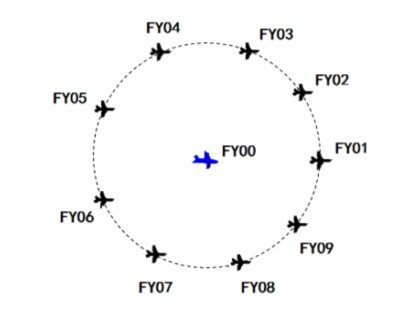
\includegraphics[width=7cm]{yuanxing.jpg}
        \caption{圆形无人机编队示意图}
        \label{yuanxing}
    \end{minipage}
    \begin{minipage}[t]{0.48\textwidth}
        \centering
        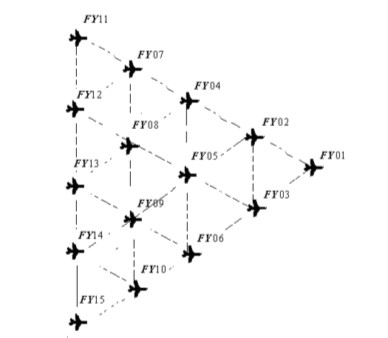
\includegraphics[width=7cm]{zhuixing.jpg}
        \caption{锥形无人机编队示意图}
        \label{zhuixing}
    \end{minipage}
\end{figure}



%----------- 二、问题分析 ---------
\section{二、问题分析}
\subsection{问题一的分析}
问题一是根据位置无偏差的发射信号无人机确定被动接受信号无人机定位的问题。对于被动接收信号无人机接收的每一个角度方位信号,在由中心无人机、发射信号无人机与被动接收信号无人机建立的三角形中。接收方位信号的角度所对应的边长固定为编队飞行的半径100m。角度与角度所对应的弦长固定,从而转化为定角定弦模型,由该模型性质可知,点的运动曲线在固定的圆周上。在具有三架发射信号无人机时可以获得两个有效的定角定弦模型,在确定两个圆时,利用接收信号信息解决圆的多解性问题。根据两个圆可以确定一个确定坐标的性质,从而求解出该点的坐标信息,从而解决无人机定位问题。

\begin{figure}[h]
    \centering
    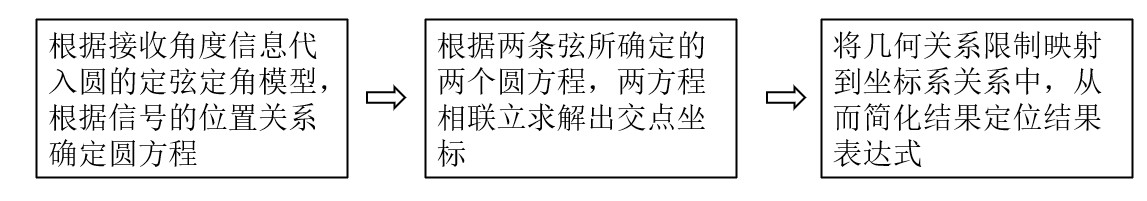
\includegraphics[width=0.8\textwidth]{liuchengtu1.jpg}
    \caption{问题一分析流程图}
    \label{liuchengtu1}
\end{figure}

\subsection{问题二的分析}

首先,我们考虑对除了FY00与FY01外仅有一架发射无人机的情况进行分析,在此情况下会出现无人机多解性的问题,说明获取的信息量还没有达到能够唯一定位的要求。因此我们增设另外一架发射信号的无人机以增加信息维度。在有四架无人机的情况下,由于FY01与FY00是固定的,因此共有28种其余两架无人机的排布方式。接着我们进行每一种情况的遍历求解,将FY00、FY01与任意一架编号未知的无人机代入问题一所建立的模型进行接收无人机的定位信息求解。考虑两次分别求解的位置信息,若两次位置信息相同,则该种方案为正确编号与正确位置信息。若在28种情况中出现一种以上的结果,则说明无人机的数量还不够,需要继续增设无人机,直至确定最少无人机数量与定位点的精确信息。

\begin{figure}[h]
    \centering
    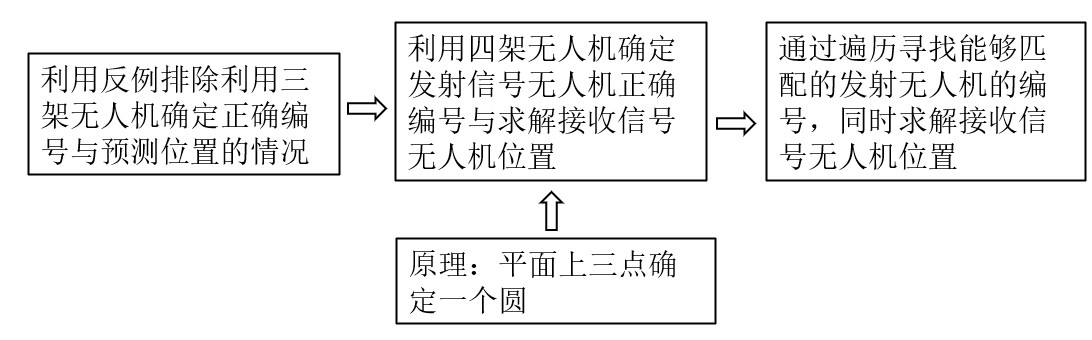
\includegraphics[width=0.8\textwidth]{liuchengtu2.jpg}
    \caption{问题二分析流程图}
    \label{liuchengtu2}
\end{figure}

\subsection{问题三的分析}
根据题目意思,在除了中央FY00无人机以外的所有无人机位置均略有偏差,需要找到调整策略使得无人机能够调整到标准编队中的正确位置。由于发射与接收无人机的位置均不准确,因此我们只能通过迭代优化的方式对无人机集群进行整体优化,使之超指向正确位置移动。由于我们需要确定无人机迭代更新的方向与距离,因此需要建立标准位置点的人工势场,根据略有偏差点的无人机获取信息角度情况确定该点在势场位置,从而沿势场梯度方向下降,更新所在位置。对于每次迭代,选取圆周上平均间隔的三个点作为信息发射的无人机,对圆周上其余6点当成接收信号无人机作位置的迭代更新,进入下一次迭代时,选取圆周上另外间隔相等的三点作为发射信号无人机,再对其余六点的位置进行迭代更新。由于无人机无法知道其余无人机是否到达正确位置,因此我们人为指定迭代次数,经过迭代次数更新后停止迭代,最后计算模型误差。

\subsection{问题四的分析}

对于问题四,本文考虑分别位于最外侧三个顶点的三架无人机所组成的等边三角形拓扑结构,假设其中两架无人机发射信号,另外一台无人机被动接收信号。对于被动接收信号的无人机,它能够接收来自发射无人机的方向信息,即$\alpha_1$角,根据$\alpha$与等边三角形内角$60°$的大小关系来进一步判断该无人机的运动。对于锥形边界上的无人机,把它们作为接收信号的无人机,去接收来自此边界上位于两个顶点无人机发射的角度信息,记作$\alpha_2$,由于边界上的无人机应与两个顶点的无人机处在同一条直线上,根据三点共线可以判断得到位于边界上的无人机应往着使$\alpha_2=180°$ 的方向进行调整。对于内部的无人机,则接收来自边界和顶点上的无人机协同发送的角度信息来进行调整。类似问题三建立的模型,改变被动接收信号的无人机,重复上面的过程进行迭代。

%----------- 三、模型假设 ----------
\section{三、模型假设}
为了对模型进行合理简化,本文给出如下假设:

1、不考虑无人机调整过程中的时间。

2、无人机在发射信号的时候无法接收信号,只有被动接收信号的无人机可以接收信号。

3、无人机的位置略有偏差假设为距离正确编队定位不超过10m

4、无人机仅能接收方位角度信息,无法测量任意两架无人机之间的距离。

5、所有无人机基于自身感知高度信息,均在统一高度飞行。

6、不考虑无人机在飞行过程中的重叠问题


%----------- 四、符号说明 ----------
\section{四、符号说明}
%使用三线表格最好~
\begin{table}[h]%htbp表示的意思是latex会尽量满足排在前面的浮动格式,就是h-t-b-p这个顺序,让排版的效果尽量好。
    \centering
    \begin{tabular}{p{2.0cm}<{\centering}p{9.0cm}<{\centering}p{2.0cm}<{\centering}}
        %指定单元格宽度, 并且水平居中。
        \hline
        符号     & 说明                             & 单位    \\ %换行 
        \hline
        $\alpha$ & 被动接收信号无人机观测角度值     & $\circ$ \\ %把你的符号写在这
        $\theta$ & 圆周上主动发送信号无人机所成夹角 & $\circ$ \\ %把你的符号写在这
        $R$ & 标准圆形无人机编队半径 & m\\
        \hline
    \end{tabular}
\end{table}


%----------- 五、模型的建立与求解 ----------
\section{五、模型的建立与求解}




\subsection{问题一:根据定角定弦模型,确定无人机定位坐标}
针对问题一,我们需要建立定弦定角的几何模型,将平面情况抽象成两个定弦定角模型的叠加,并计算两个轨迹圆的正确解析方程,将两个圆的方程表达式相联立,最后求解出该点在平面坐标系下的坐标,实现接收信息无人机的准确定位。由题目信息可知,发射信号的无人机的位置无偏差,因此如图\ref{sizhong}可知,处于圆心处的FY01与圆周上的其他两家无人机的位置共有四种分布情况,分别对应圆心角为$0^{\circ}$、$40^{\circ}$、$80^{\circ}$、$160^{\circ}$,其余位置的情况均可以通过旋转与翻转转化为如图所示的四种情况。因此,我们将圆心角进一步抽象为$\theta$进行问题的求解。


\begin{figure}[h]
    \centering
    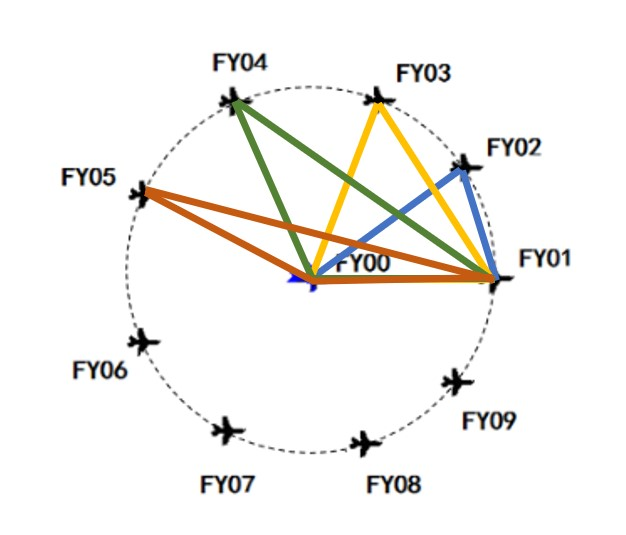
\includegraphics[width=0.5\textwidth]{sizhong.jpg}
    \caption{发射信号无人机方位的四种情况}
    \label{sizhong}
\end{figure}

\subsubsection{模型的建立}

如图\ref{qingkuang1}所示,对于固定长度的BC段直线。若A点与B、C两点所成的角度恒为一个定值$\alpha$,那么点A运动的轨迹在一个圆上。根据正弦定理可以得到轨迹圆的半径$R$:
\begin{equation}
    \frac{BC}{sin(\alpha)} = 2R
\end{equation}

其中BC为BC线段的长度,R为A形成轨迹圆的半径。

在固定BC线段的条件下加入坐标系,定弦定角会出现如图\ref{qingkuang1}与\ref{qingkuang2}的两种情况,即移动的点A位于固定弦BC的上方与下方,若B点为坐标系原点,则对应圆心的纵坐标会出现正值与负值两种情况。在后续求解过程中会对轨迹圆的解析式产生影响。



\begin{figure}[htbp]
    \centering
    \begin{minipage}[t]{0.48\textwidth}
        \centering
        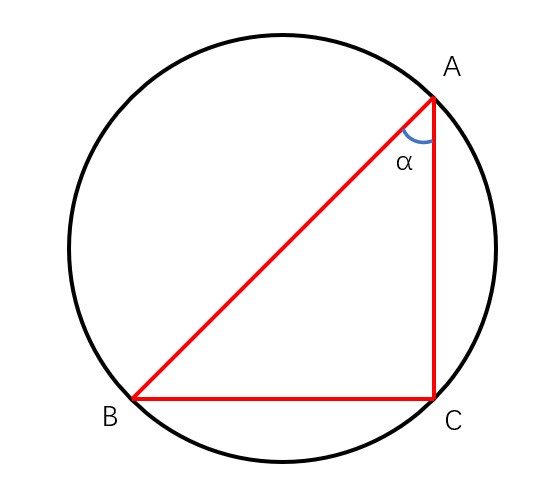
\includegraphics[width=5cm]{dingxiandingjiao.jpg}
        \caption{定弦定角模型情况一}
        \label{qingkuang1}
    \end{minipage}
    \begin{minipage}[t]{0.48\textwidth}
        \centering
        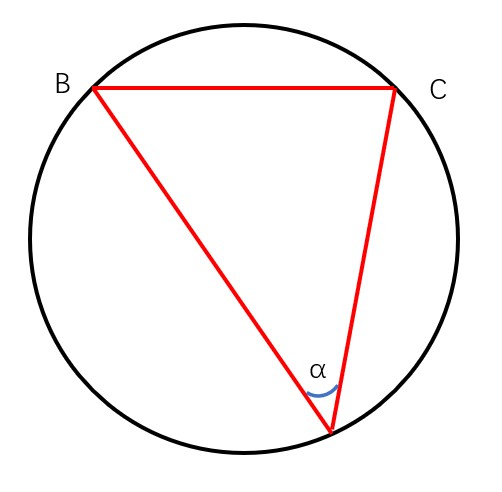
\includegraphics[width=5cm]{dingxiandingjiao2.jpg}
        \caption{定弦定角模型情况二}
        \label{qingkuang2}
    \end{minipage}
\end{figure}

如图\ref{moxing1},根据题意,假设圆周上的两家发射信号无人机分别为FY0X与FY0Y,两架无人机所成角度为$\theta$。FY00与FY0X、FY00与FY0Y之间的距离均为标准编队中的半径100m。在被动接收信息无人机端,观测的FY0X与FY00之间的夹角为$\alpha_1$,观测的FY00与FY0Y之间的夹角为$\alpha_2$。因此,建立模型1为两个定弦定角模型的叠加。



\begin{figure}[h]
    \centering
    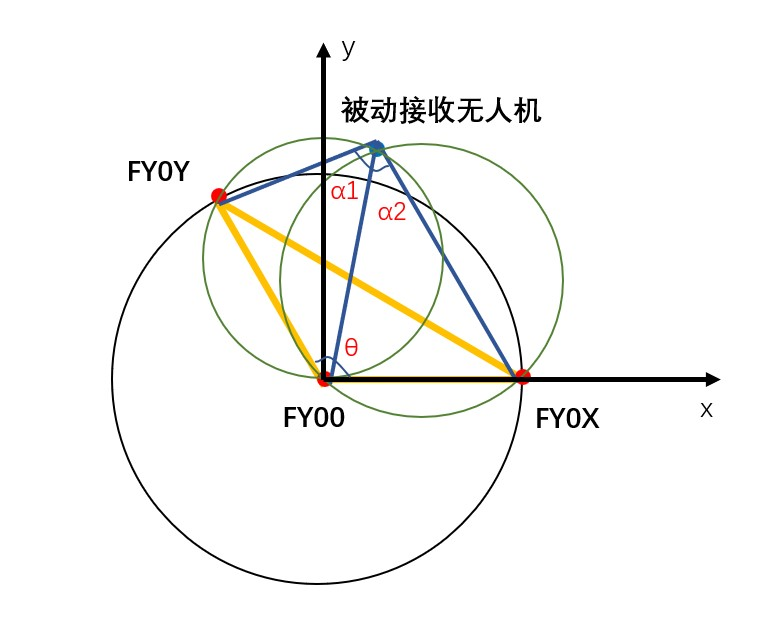
\includegraphics[width=0.5\textwidth]{yuan.jpg}
    \caption{问题一建立的模型}
    \label{moxing1}
\end{figure}

以FY00与FY0X所在直线为x轴,以FY00与FY0Y所在直线为y轴,在平面上建立平面直角坐标系。我们分别考虑两个轨迹圆,并分析各轨迹圆属于两个两种情况中的哪种情况,赋予正确的解析坐标式。由观测到的$\alpha_1$、$\alpha_2$、$\alpha_3$的相对位置和大小关系可以确定被动接收信息无人机在弦的上方还是下方,从而解决圆的多解问题,在被动接收信息无人机中分析信息来源:

(1)若FY00的信息来源位于FY01的顺时针方向,则由FY0Y、FY00、被动接收信号无人机所构成的轨迹圆的方程为:
\begin{equation}
    (x - \frac{50\sin(\theta + \alpha_1)}{\sin(\alpha_1)})^2 + (y + \frac{50\cos(\theta + \alpha_1)}{\sin(\alpha_1)})^2 = (\frac{50}{\sin(\alpha_1)}) ^ 2
    \label{yuan1}
\end{equation}

(2)若FY00的信息来源位于FY01的逆时针方向,则由FY0Y、FY00、被动接收信号无人机所构成的轨迹圆的方程为:
\begin{equation}
    (x + \frac{50\sin(\theta - \alpha_1)}{\sin(\alpha_1)})^2 + (y - \frac{50\cos(\theta - \alpha_1)}{\sin(\alpha_1)})^2 = (\frac{50}{\sin(\alpha_1)}) ^ 2
    \label{yuan2}
\end{equation}

(3)若FY00的信息来源位于FY01的逆时针方向,则由FY0Y、FY00、被动接收信号无人机所构成的轨迹圆的方程为:
\begin{equation}
    (x - 50) ^{2} + (y - \frac{50}{\tan(\alpha_{2})}) ^ {2} = (\frac{50}{\sin(\alpha_2)}) ^ 2
    \label{yuan3}
\end{equation}


(4)若FY00的信息来源位于FY01的逆时针方向,则由FY0Y、FY00、被动接收信号无人机所构成的轨迹圆的方程为:
\begin{equation}
    (x - 50) ^{2} + (y + \frac{50}{\tan(\alpha_{2})}) ^ {2} = (\frac{50}{\sin(\alpha_2)}) ^ 2
    \label{yuan4}
\end{equation}


\subsubsection{模型的求解}
通过定弦定角模型所确定的两个轨迹圆组合共有4种情况,因此我们选择公式\ref{yuan1}与公式\ref{yuan3}所确定的轨迹圆进一步分析两圆交点解的计算。

\begin{figure}[h]
    \centering
    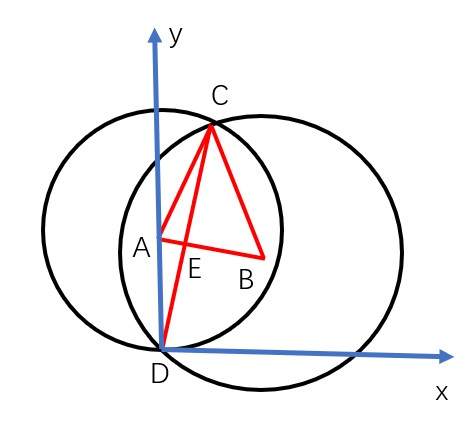
\includegraphics[width=0.3\textwidth]{liangyuan.jpg}
    \caption{两个圆的交点模型}
    \label{jiaodian}
\end{figure}

记两个轨迹圆的圆心为$(x_1,y_1)$与$(x_2,y_2)$,可以得到:
\begin{equation*}
    (x_1, y_1) = (50,\frac{50}{\tan(\alpha_2)})
\end{equation*}
\begin{equation*}
    (x_2, y_2) = (\frac{50\sin(\theta + \alpha_1)}{\sin(\alpha_1)}, - \frac{50\cos(\theta + \alpha_1)}{\sin(\alpha_1)})
\end{equation*}

记$K_1$为两个圆心连线形成直线的斜率,可以得到:
\begin{equation}
    \begin{cases}
        K_1 = \frac{y_2 - y_1} {x_2 - x_1} = =\dfrac{\sin \alpha_{1}\cos \alpha _{2}+\sin \alpha _{2}\cos _{}\left( \theta +\alpha _{1}\right) }{\sin \alpha _{2}\left( \sin \alpha_{1}-\sin \left( \theta +\alpha_{1}\right) \right) } \\
        \\
        K_2 = -\frac{1}{K_1} = -\dfrac{1}{K1}=\dfrac{\sin \alpha _{2}\left( sin\left( \theta +\alpha _{1}\right) -\sin \alpha _{1}\right) }{\sin \alpha_{1}\cos \alpha _{2}+\sin \alpha _{2}\cos \left( \theta +\alpha _{1}\right) }    \\
        \\
        L = AB = \sqrt{(x_1 - x_2) ^ 2 + (y_2 - y_1) ^ 2}
    \end{cases}
\end{equation}


又由几何关系
\begin{equation}
    \begin{cases}
        CE ^{2} = r_1 ^{2} - AE ^{2} \\
        CE ^{2} = r_2^{2} - EB ^{2}  \\
        EB ^{2} = (L - AE) ^{2}      \\
    \end{cases}
\end{equation}

解得:
\begin{equation*}
    AE = \frac{(r_1 ^2 - r_2 ^2 + L ^2)}{2L}
\end{equation*}

从而得到E点坐标:
\begin{equation}
    \begin{cases}
        x_0 = x_1 + \frac{AE}{L} (x_2 - x_1) \\
        y_0 = y_1 + \frac{AE}{L} (y_2 - y_1)
    \end{cases}
\end{equation}

由于D点所处位置为圆心,因此交点C的坐标为E坐标的两倍,即为:
\begin{equation}
    \begin{cases}
        x_c = 2(x_1 + \frac{AE}{L} (x_2 - x_1)) \\
        y_c = 2(y_1 + \frac{AE}{L} (y_2 - y_1)) \\
    \end{cases}
\end{equation}



最后根据所选取的无人机编号差可以确定所形成的圆圆心角确定$\theta$的值,$x_c$与$y_c$中的参数$x_1$、$AE$、$L$均在公式(6)-(8)中利用$\alpha_1$、$\alpha_2$与$\theta$来表示。从而将所有的参数代入表达式中,可以确定最后的接收信号无人机的定位。

\subsection{问题二:遍历优化算法解决在发送无人机编号未知情况下接收信号无人机方位解算问题}
\subsubsection{模型的建立}
首先,我们对除了FY00与FY01的发射信号无人机仅有一架的情况进行建模分析。

如图\ref{sandian}所示,固定FY00与FY01两点,对剩余的8个点进行遍历分析,FY00、FY01、任一发射信号无人机便成为已知条件。对于三个已经确定编号的无人机,可以代入问题一种所建立的定位模型。接收无人机所接收到的方位信息固定,利用情况枚举来确认是否有多解性的可能。图中与每一个蓝点连线的红点代表经过模型一后输出的接收信号无人机的坐标。从图中可知,通过选用不同编号的无人机,对应的预测点有多重情况且无法被排除。因此仅有三架无人机的模型缺少信息维度,无法准确确定目标无人机位置。

\begin{figure}[h]
    \centering
    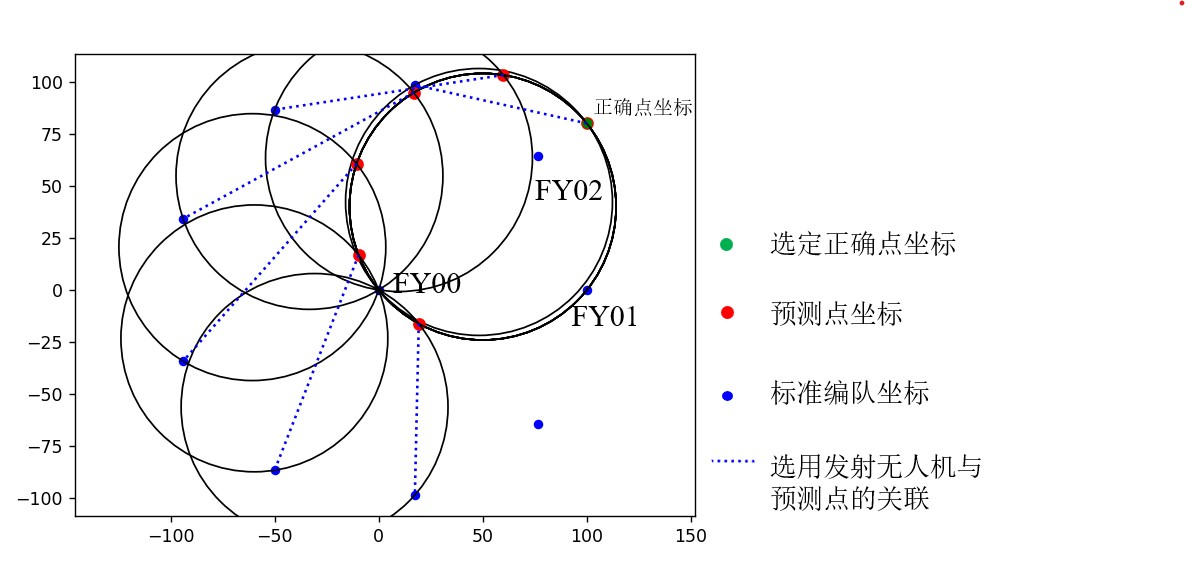
\includegraphics[width=0.8\textwidth]{sandian.jpg}
    \caption{基于3架无人机出现多解的情况}
    \label{sandian}
\end{figure}

在排除三架无人机实现准确定位情况的背景下,我们选用四架无人机发射信号,即选用FY00、FY01与圆周上任意选取两个编号未知的无人机来接收消息。在圆周上选用两个编号未知的无人机共有$C_{8}^{2}=28$种情况。

\begin{figure}[h]
    \centering
    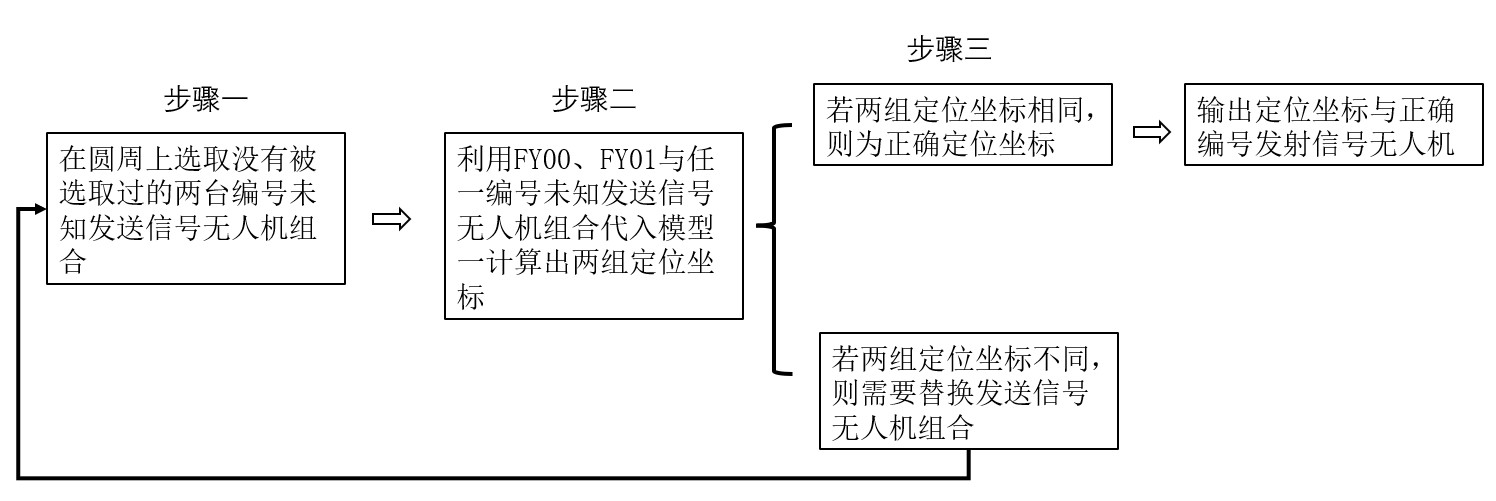
\includegraphics[width=1\textwidth]{wenti2liucheng.jpg}
    \caption{模型二流程图}
    \label{moxing2liucheng}
\end{figure}

如流程图\ref{moxing2liucheng}所示,根据平面上三个不重叠且相交的圆唯一确定一个点的定理,我们通过遍历28种可能情况,可以得到四个圆,利用圆所确定点的相交性确定正确点的坐标与正确编号组合:

\textbf{步骤一:在圆周上任意选取两个无人机作为发射信号无人机}

如图\ref{moxing2}所示,从圆周上任意选取两台无人机(除去已经选择的FY01)共有28种情况,假设选取的无人机的编号为FY0X与FY0Y。

\begin{figure}[h]
    \centering
    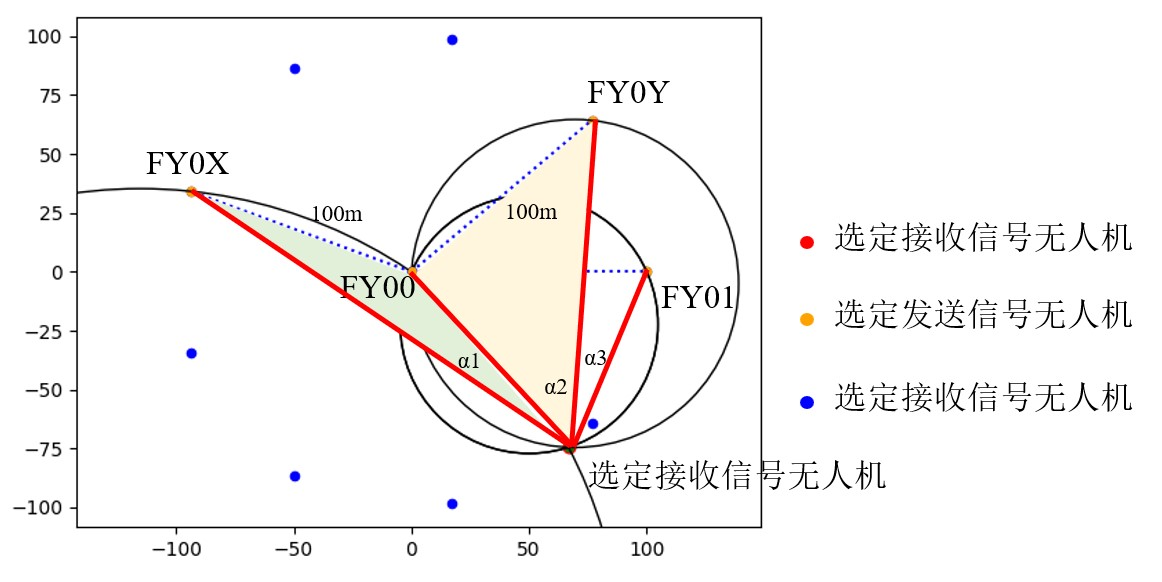
\includegraphics[width=0.6\textwidth]{wenti2.jpg}
    \caption{模型二}
    \label{moxing2}
\end{figure}

\textbf{步骤二:利用模型一求解预测坐标}

当选定发射无人机的编号时,场景中的无人机共构成两组模型一。我们将4架无人机组合成FY00、FY01、FY0X的组合与FY00、FY01、FY02的组合。由于无人机接收到的角度方位信息确定,因此利用问题一中求解出的定弦定角模型一可以求解出预测无人机在全局位置信息:

FX00、FY01、FY0X所构建的模型一的角度信息为$\alpha_1$,由于编号FY01与FY0X已知,因此可以通过模型一求解出预测点一位置记为:

\begin{equation}
    (x_{p1}, y_{p1}) = Model_1(FY00, FY0X, \alpha_1)
\end{equation}

FX00、FY01、FY0Y所构建的模型一的角度信息为$\alpha_2$,由于编号FY01与FY0Y已知,因此可以通过模型一求解出预测点位置记为:

\begin{equation}
    (x_{p2}, y_{p2}) = Model_1(FY00, FY0Y, \alpha_2)
\end{equation}

\textbf{步骤三:对比两组预测位置,确定预测无人机真实位置}

比较步骤二解算出的位置信息,若位置信息相同,即

\begin{equation}
    \begin{cases}
        x_{p1} = x_{p2}\\
        y_{p1} = y_{p2}\\
    \end{cases}
\end{equation}

则该点为正确编号的无人机组合所计算出的接收信号无人机的定位信息。

如果两者位置信息不相同,则说明选取的无人机组合不正确,需要重新进入步骤一选取其余未尝试过的无人机编号组合,直至求解出正确的编号组合。\\

\subsubsection{模型的验证}

\begin{figure}[h]
    \centering
    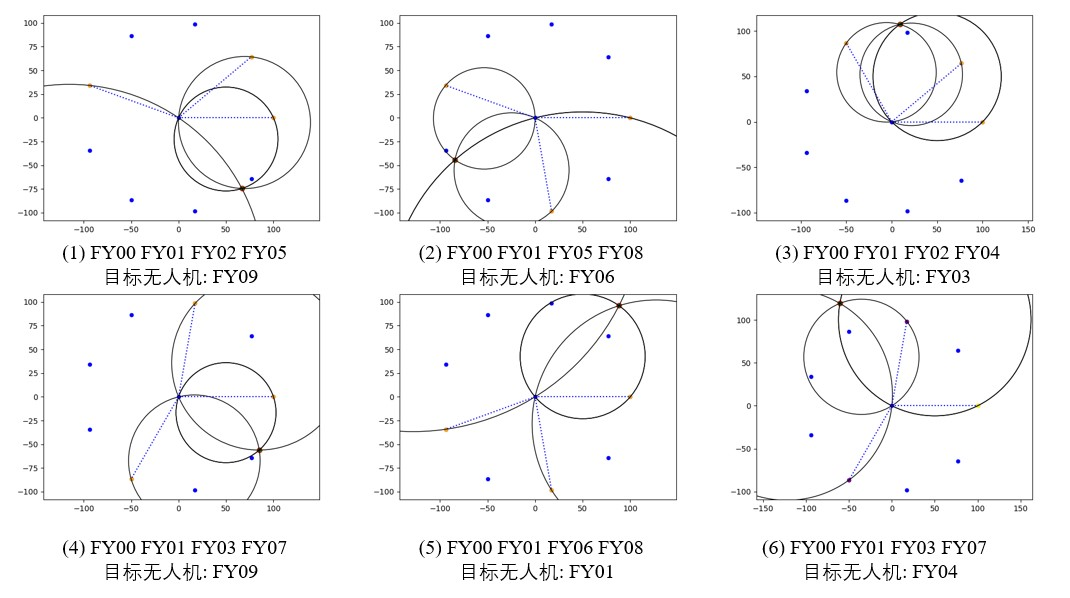
\includegraphics[width=1\textwidth]{duoqingkuang.jpg}
    \caption{模型二中验证不同情况示意图}
    \label{duoqingkuang}
\end{figure}

\textbf{步骤一:建立验证模型}

我们随机选取一架圆周上的无人机并对无人机进行位置在标准编队附近随机偏移处理,作为位置略有偏差的无人机A。对于选取的点,我们规定无人机在横纵坐标偏移为$\pm6m$的矩形区间内进行随机数偏移。

接着在圆周上选取其余两架无人机作为编号未知的发射信息无人机,记为FY0X与FY0Y。计算A与FY0X与FY0Y的夹角角度作为已知的角度信息。\\

\textbf{步骤二:利用验证模型进行模型检验}

在验证阶段,将角度信息代入上述建立模型,如图\ref{duoqingkuang}所示为部分不同情况的示意图,图中橙色点代表随机选取的编号未知的无人机,蓝色点代表,而绿色点与红色点重合就代表选取接收信息的无人机的定位与仅通过角度信息经过模型输出的定位坐标相重合。

同时我们也验证1000组不同情况,最终得出结果均能与模型假设匹配。



\subsection{问题三:利用优化人工势场模型迭代解决无人机位置调整问题}


\begin{figure}[h]
    \centering
    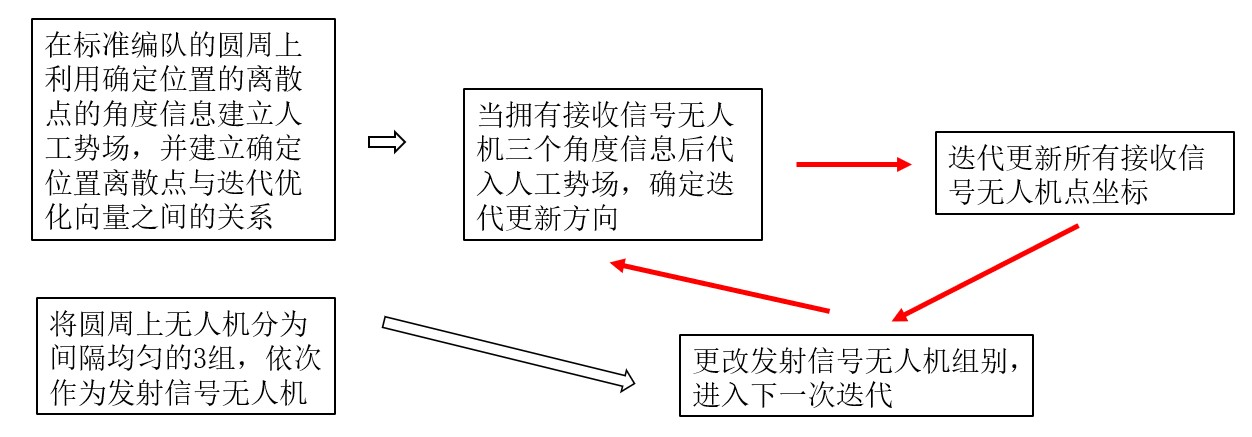
\includegraphics[width=1\textwidth]{wentisan.jpg}
    \caption{模型三流程图}
    \label{moxingsan}
\end{figure}

在除了FY00以外的无人机位置均有偏差的情况下,无法利用距离信息进行无人机确切位置的解算,由于只有角度信息,没有距离信息。因此缺少必要条件数量,只考虑优化模型对接收信号无人机进行位置的最优化处理。

本文需要构建迭代优化模型,对无人机集群整体进行调整。在模型的每一次迭代过程中,需要确定迭代的目标与在当前状态下模型迭代的方向。由于有效信息仅有三个角度方位,因此需要构建势场模型将三个角度映射到势场三维空间中的坐标点。通过势场的梯度信息确定模型的迭代方向,再将模型迭代方向从势场中映射回二维的平面集合空间,从而确定无人机的飞行方向。

由于在问题三中用于构建势场的无人机并非处于标准编队位置,因此我们需要在每次移动无人机的时候改变发射信号无人机的编号,从而实现所有无人机位置的更新,具体模型与算法实现原理如下:

\subsubsection{建立标准位置的势场模型}

\textbf{第一部分:人工势场原理分析}

人工势场包括引力场与斥力场,其中目标点对物体产生引力,引导物体朝向目标点运动;而障碍物对物体产生斥力,避免物体与之相撞,物体在路径上每一点的受力均为引力场与斥力场对物体吸引力的合力。\cite{kownacki2017local}

对于引力场而言,常用的引力场函数为
\begin{equation}
    U_{att}(q) = \frac{1}{2} \xi \rho^{2} (q, q_{goal}) 
\end{equation}

其中,$\xi$是尺度因子,$\rho(q, q^2)$ 代表物体当前状态与目标位置之间的距离。

有了引力场,物体受到的引力记为引力场的导数
\begin{equation}
    F_{att}(q) = -\nabla U_{att}(q)
\end{equation}

在本问题中,由于飞机可以向任意方向移动,故不存在障碍物,也就不存在斥力场的影响。\cite{张鲲2018海上侦察船的纯方位无源定位技术研究}\\

\textbf{第二部分:改进优化人工势场的机理分析}

根据无人机仅能接收到角度信息,没有方位定位信息的题目条件,经过测试无法通过足够有效的约束条件,直接进行人工势场方程构建势场的函数。因此我们提出基于改进优化人工势场的模型,该模型基于离散数据点信息,并对离散数据点中间的区域进行二维线性差值处理。从而模拟人工势场,让无人机在通过接收无人机三个角度信息的情况下能够通过差值拟合函数求取迭代更新方向与距离,从而实现无人机位置的一次迭代。\\

\textbf{第三部分:人工势场分区分点构建}


\begin{figure}[htbp]
    \centering
    \begin{minipage}[t]{0.48\textwidth}
        \centering
        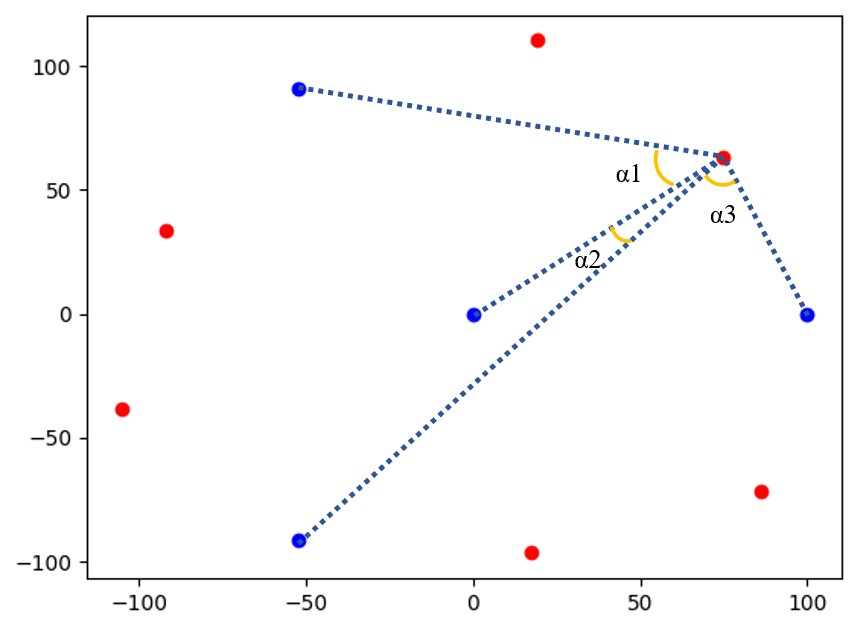
\includegraphics[width=5cm]{qudian.jpg}
        \caption{观测角度示意图}
        \label{qudian}
    \end{minipage}
    \begin{minipage}[t]{0.48\textwidth}
        \centering
        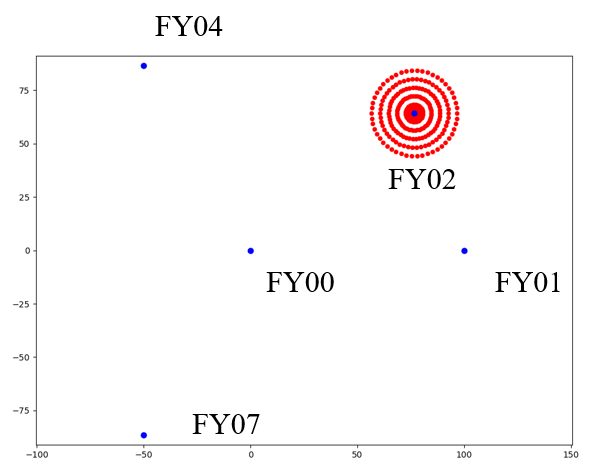
\includegraphics[width=5cm]{fenqu.png}
        \caption{在标准编队位置周围构建分区与分点}
        \label{fenqu}
    \end{minipage}
\end{figure}


首先,将接收信息无人机所收集的三个角度方位信息转化为空间中$R^3$中的坐标,如图\ref{qudian}所示,我们将$\alpha_1$、$\alpha_2$、$\alpha_3$的坐标作为空间中三维坐标点$(x_{\alpha},y_{\alpha},z_{\alpha})$。

然后,如图\ref{fenqu}所示,针对标准编队(即9架无人机均匀分布在半径为100m的圆周上)所形成的圆周的每一个点,我们分别在每一个点处以0米、0.5米、1米、2米、4米、8米、12米、16米、20米为半径形成的圆周上取点,并搜集有效角度信息,将此角度信息以上述方式映射至三维空间$R^{3}$中,记录该点的最优更新方向,形成如图\ref{3d}所示的以角度信息构建的人工势场点云模型。


\begin{figure}[htbp]
    \centering
    \begin{minipage}[t]{0.48\textwidth}
        \centering
        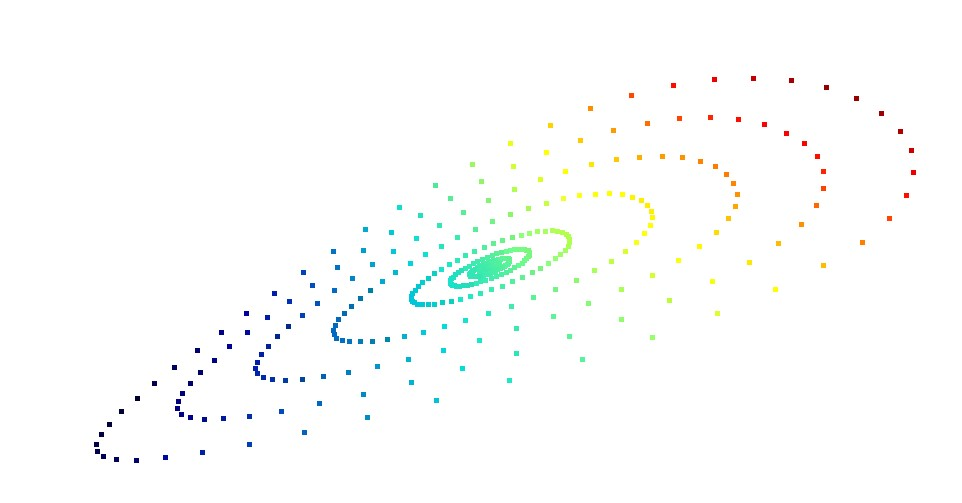
\includegraphics[width=5cm]{3d.jpg}
        \caption{通过角度构建的人工势场点云模型}
        \label{3d}
    \end{minipage}
    \begin{minipage}[t]{0.48\textwidth}
        \centering
        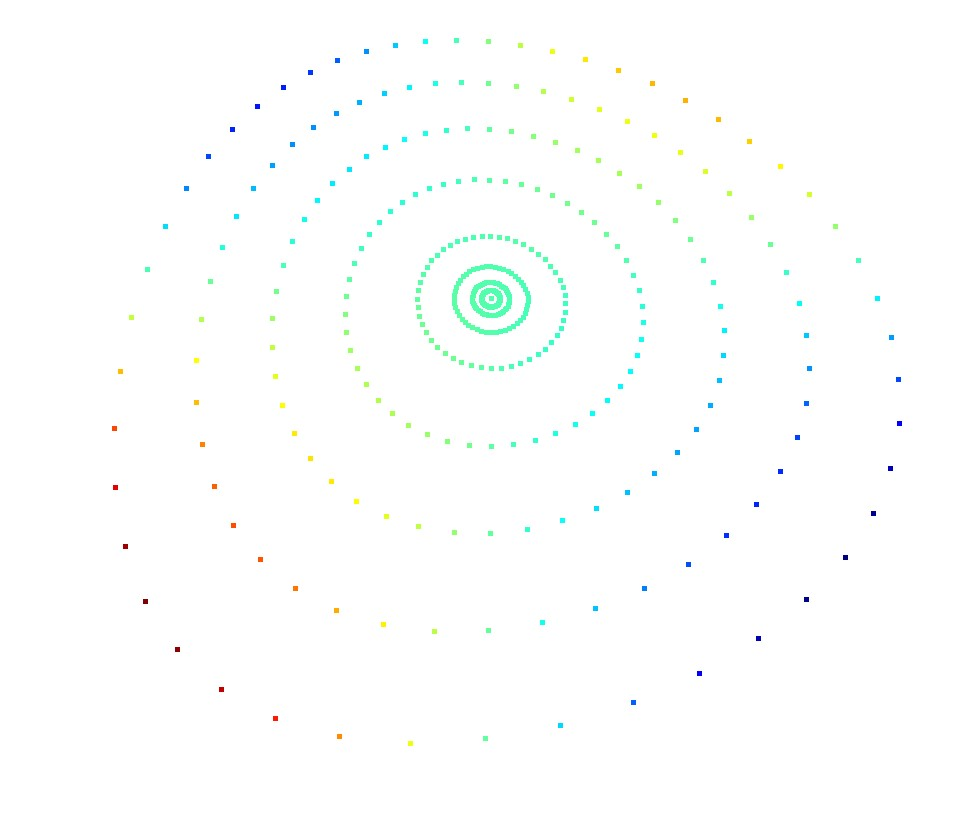
\includegraphics[width=5cm]{3dn.jpg}
        \caption{经过仿射变化调整后的人工势场点云模型}
        \label{3dn}
    \end{minipage}
\end{figure}

\textbf{第四部分:迭代更新向量的计算}

根据二维线性差值原理,我们需要在映射空间中寻找与$(x_{\alpha}, y_{\alpha}, z_{\alpha})$最近的四个点,并将此四点在极坐标系中指向中心的向量加权平均得到迭代更新向量。

\begin{figure}[h]
    \centering
    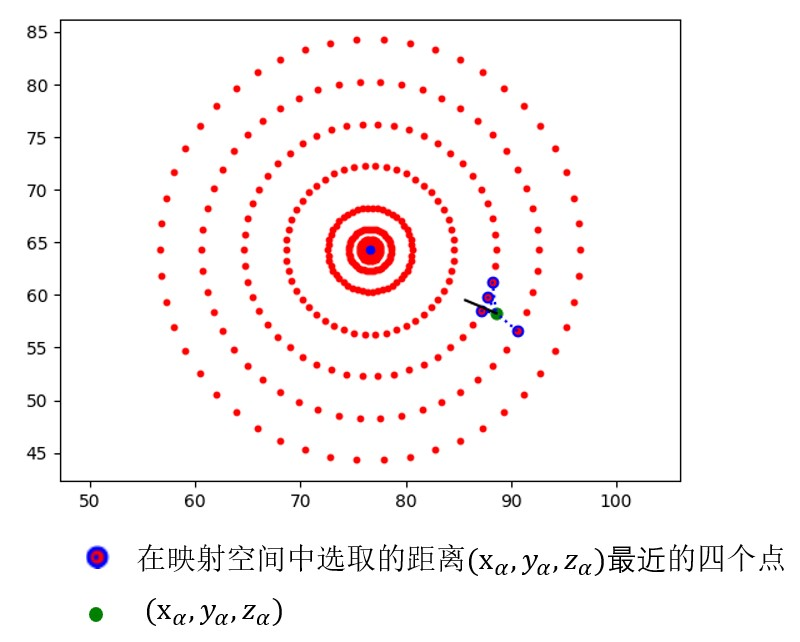
\includegraphics[width=0.4\textwidth]{sigedian.jpg}
    \caption{通过距离最近四点计算迭代更新向量示意图}
    \label{sigedian}
\end{figure}

由于需要做二维线性差值,因此需要将图\ref{3d}中的点云和横轴与纵轴进行归一化处理,通过三维空间中仿射基底变化实现:


设$E_1,E_2$为两个维度相同的几何向量空间,称从$E_1$到$E_2$的一个映射为仿射映射,若该映射是由一个非奇异的线性变换和一个平移变换所组成。\\
  设$X_1\in E_1,X_2\in E_2,A\in M_{n}(\mathbb{R})$,$b\in M_{n,1}$为平移变换列矩阵,其中n为向量空间的维度。那么从从$E_1$到$E_2$的一个仿射映射可以记作\\
  \begin{equation}
    X_1 = AX_2 + \mathbf{b}
    \label{funshe1}
  \end{equation}


由三维空间的仿射变换公式可以写成如下的矩阵表示形式:
$$
 \begin{pmatrix}
    x_{1} \\
    y_{1} \\
    z_{1} \\
    1     \\
  \end{pmatrix} 
    = \begin{pmatrix}
    a_{11} & a_{12} & a_{13} & b_1\\
    a_{21} & a_{22} & a_{23} & b_2\\
    a_{31} & a_{32} & a_{33} & b_3\\
    0 & 0 & 0 & 1\\
  \end{pmatrix}
  \begin{pmatrix}
    x_{2} \\
    y_{2} \\
    z_{2} \\
    1     \\
  \end{pmatrix}
$$

对于本模型而言,通过比较最外层点云两两之间的距离可得到两个点的最长距离,以此两个点为端点构建向量$\overrightarrow{MaxVec}$;得到两个点的最短距离,以此两个点为端点构造向量$\overrightarrow{MinVec}$,以此两个向量与平面法向量$\vec{n}$组成的基底与标准坐标系的基底进行基底过渡矩阵计算,$b$的向量即为从选定的FY0X指向$(0,0,0)$的向量:
$$
    A =
    \begin{pmatrix}
            \overrightarrow{MinVec}\\
            \overrightarrow{MaxVec}\\
            \vec{n} \\
    \end{pmatrix}, \quad
    b = \begin{pmatrix}
        x_{FY0X}\\
        y_{FY0X}\\
        z_{FY0X}\\
    \end{pmatrix}
$$

经过处理后得到如图\ref{3dn}所示的标准映射空间。在此空间中需要寻找$(x_{\alpha}, y_{\alpha}, z_{\alpha})$距离最近的四个点,采用KD树模型的方法进行求解:

\textbf{针对本模型构建$KD-tree$的原理}

已知人工利用角度信息构建的三维映射空间中无序化的3维点云,每一个点云节点都是3维的数据。

1、初始化分割轴:分别计算被接受信号无人机周围的点$(\alpha_x,\alpha_y,\alpha_z)$对应 $x,y,z$ 坐标角度信息的方差(下面以$x$轴方向上的数据计算方差为例)
$$
s^2 = \frac{\sum_{i=1}^2(\alpha_{xi}-\overline{\alpha_{x}})^2}{n}
$$
取具有最大方差的坐标轴作为初始分割轴,记作$r_1$;

2、确定分割节点:对现有的角度信息按照分割轴维度进行检索,将角度信息从小到大排序后选出中位数数据,并将其当作是分割点,这个节点的分割平面就是通过该点并垂直于具有最大方差坐标轴的一个二维平面。

3、划分双子空间:在当前分割轴中,所有小于中位数的角度信息全部划分到左子空间中;在当前分割轴中,所有大于等于中位数的角度信息全部划分到右子空间中。

4、更新分割轴:利用公式$r = (r+1) $ \% $n$ 求出此三维映射空间中的新分割轴。

5、确定子节点:在左子空间的角度信息中进行步骤2确定左子节点;在右子空间的数据中进行步骤2确定右子节点。

同时将子空间和角度信息进一步划分, 如此反复进行上述步骤直到子空间中只包含一个角度信息点$(\alpha_x,\alpha_y,\alpha_z)$。

这样一来就可以将整个三维映射空间划分成了若干个子空间。考察被接收信号的无人机映射到此空间上的坐标$(\alpha_1,\alpha_2,\alpha_3)$,以该坐标为中心点,利用$KD-tree$向周围附近空间进行检索,便可找到距离坐标$(\alpha_1,\alpha_2,\alpha_3)$最近的其它四个点的坐标。


通过这四点的坐标,根据在建立人工势场时存储的迭代更新向量可以寻找到对应的四个最近点的的迭代更新向量,记为$\bar v_1 \quad \bar v_2 \quad \bar v_3 \bar v_4$。因此,针对$(x_{\alpha} , y_{\alpha} , z_{\alpha})$所构建的迭代更新向量为:
\begin{equation}
    \overrightarrow{\Delta v} = (\bar v_1 + \bar v_2 + \bar v_3 + \bar v_4)/ 4
\end{equation}





\subsubsection{无人机位置迭代策略}

由于圆周上9架无人机的位置均不准确,因此在迭代更新的过程中,每一架无人机均需要更新位置。因此,需要制定合理迭代策略以满足模型收敛需求。\\

\textbf{步骤一:确定发射信号无人机编号}

根据题意,接收信号无人机仅能接收到发送信号无人机的方位角度信息。考虑到势场建立所需要的角度信息对称性,我们在选取发射信号无人机编号时同样考虑模型的对称性。因此,我们将圆周上的9架无人机划分为3组,分别是:

\begin{table}[h]%htbp表示的意思是latex会尽量满足排在前面的浮动格式,就是h-t-b-p这个顺序,让排版的效果尽量好。
    \centering
    \caption{圆周上无人机分组表}
    \begin{tabular}{p{2.0cm}<{\centering}p{9.0cm}<{\centering}p{2.0cm}<{\centering}}
        %指定单元格宽度, 并且水平居中。
        \hline
        组合编号     & 发射信号无人机编号                         \\
        \hline
        A组 &  FY00、FY01、FY04、FY07   \\ %把你的符号写在这
        B组 &  FY00、FY02、FY05、FY08 \\
        C组 &  FY00、FY03、FY06、FY09 \\
        \hline
    \end{tabular}
\end{table}

\textbf{步骤2:接收信号无人机获取角度信息,计算迭代更新向量}

当有4台发射信号无人机时,圆周上其余6台为接收信号无人机。每一台接收信号无人机根据自己的获取的3个角度信息,通过代入5.3.1节中讨论的优化人工势场模型确定各自的迭代更新变量$\Delta v = (\Delta \rho, \Delta \theta)$,在接受信号无人机端的自身极坐标下更新坐标。

\textbf{步骤3:更换圆周无人机组别,继续进行迭代}

在一次迭代过后,接受信号无人机在发射信号无人机的观测条件下已经达到最优情况,然而发射信号无人机的位置略有偏差,因此我们需要更换发射信号的无人机使得接收信号无人机与发射信号无人机之间能够相互迭代,以达到全局均为最优解的情况。

目标函数为:
\begin{equation}
    F(x) = \Sigma^{9}_{i = 0} \left\lvert R_{FY0i} - \bar R\right\rvert 
    \quad \bar R = \frac{\Sigma^{9}_{i = 0}R_{FY0i}}{9}
\end{equation}
其中,$x$为迭代次数,$\bar R$为圆周上点的平均半径

因此我们按照A组->B组->C组->A组的顺序循环迭代,使得每一次都更新不同架次的无人机,从而达到全局最优,目标函数最小化。

\begin{figure}[h]
    \centering
    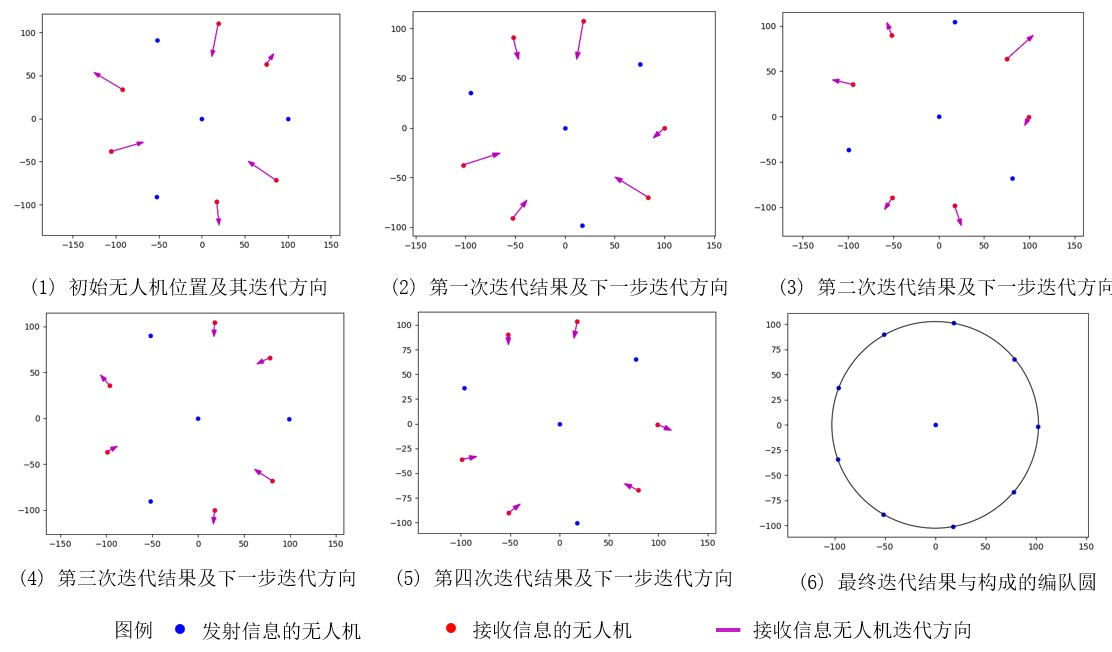
\includegraphics[width=1\textwidth]{diedai.jpg}
    \caption{无人机位置调整迭代过程图(为增强模型可视化,箭头长度增长10倍)}
    \label{diedai}
\end{figure}


\subsubsection{无人机位置迭代求解过程}
将题目中给定的所有无人机的初始位置位置进行建模,通过角度计算可得出各接收信息无人机所接收到的三个角度信息。

将角度信息代入无人机迭代更新模型,求解如出表\ref{table2}所示的无人机位置更新向量。其中,表\ref{table2}中的向量为基于接收信息无人机极坐标系的更新向量。

将更新向量代入上述建立的迭代更新方案模型,求解出如图\ref{diedai}所示的迭代更新方案。

最终迭代10次即可获得目标函数误差小于0.5的结果,迭代50次可以获得目标函数误差小于0.3的结果。



\begin{table}[h]%htbp表示的意思是latex会尽量满足排在前面的浮动格式,就是h-t-b-p这个顺序,让排版的效果尽量好。
    \centering
    \caption{模型迭代次数与各无人机更新迭代向量(极坐标)关系表}
    \begin{tabular}{p{1.0cm}<{\centering}p{2.3cm}<{\centering}p{2.3cm}<{\centering}p{2.3cm}<{\centering}p{2.3cm}<{\centering}p{2.3cm}<{\centering}}
        %指定单元格宽度, 并且水平居中。
        \hline
        迭代     & 1 & 2 & 3& 4 &   5  \\
        \hline
        $FY00$ & $ (0.000, 0.000) $& $(0.000, 0.000)$& $(0.000, 0.000)$& $(0.000, 0.000)$ &$(0.000, 0.000)$\\
          $FY01$ & $ (0.000, 0.000) $&  $(0.789, 110.8)$& $(0.791,131.1)$ &$(0.000, 0.000)$ &$(0.316, 216.8)$\\
           $FY02$ & $ (3.167, 260.1) $& $(0.000, 0.000)$& $(0.556,27.8)$& $(0.790, 10.89)$ &$(0.000, 0.000)$\\
            $FY03$ & $ (1.583, 283.7) $& $(1.575,167.1)$& $(0.000, 0.000)$& $(0.790, 37.04)$ &$(0.449, 288.1)$\\
             $FY04$ & $ (0.000, 0.000) $& $(0.790, 237.0)$& $(0.791, 264.6)$& $(0.000, 0.000)$ &$(0.317, 345.2)$\\
              $FY05$ & $ (3.158, 17.87) $& $(0.000, 0.000)$& $(1.585, 146.9)$& $(0.792, 154.5)$ &$(0.000, 0.000)$\\
               $FY06$ & $ (1.583, 52.17) $& $(1.582, 289.1)$& $(0.000, 0.000)$& $(0.791, 337.4)$ &$(0.791, 24.29)$\\
                $FY07$ & $ (0.000, 0.000) $& $(0.317, 244.4)$& $(0.792, 205.9)$& $(0.000, 0.000)$ &$(0.236, 39.90)$\\
                 $FY08$ & $ (3.167, 148.6) $& $(0.000, 0.000)$& $(0.792, 267.6)$& $(0.996, 258.9)$ &$(0.000, 0.000)$\\
                   $FY09$ & $ (0.792, 222.4) $& $(3.157, 41.86)$& $(0.000, 0.000)$& $(0.317, 272.1)$ &$(0.316, 198.5)$\\
             
        \hline
    \end{tabular}
    \label{table2}
\end{table}





\subsubsection{无人机位置迭代结果分析}

\begin{figure}[h]
    \centering
    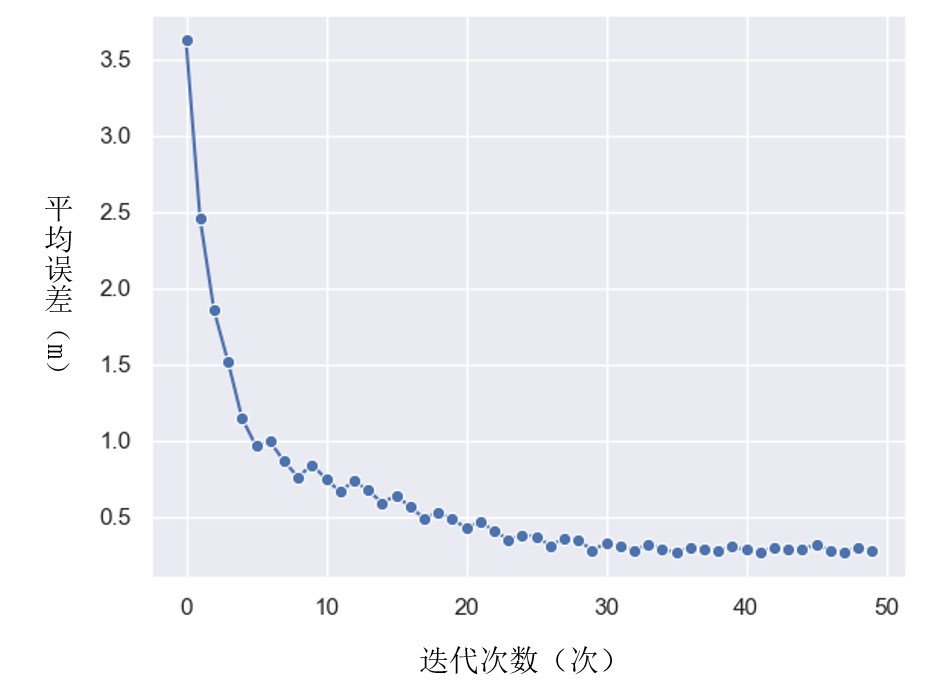
\includegraphics[width=0.5\textwidth]{wucha.jpg}
    \caption{无人机位置迭代中平均误差与迭代次数关系图}
    \label{wucha}
\end{figure}
图\ref{wucha}的横坐标是算法模型迭代的次数,纵坐标是每一次迭代过程中,圆周点与所形成的拟合圆的平均误差。


图\ref{wucha}所示的结果为对这个算法模型迭代50次时的误差值F(x)(见公式(17))。从图中可以发现此算法在前6次迭代过程中,误差下降的速率非常快,从3.622m直接下降到了0.922m。说明该算法模型可以在迭代次数很小时就表现出强的收敛性,这是该算法的优点。可以看到,在经过20次迭代后可以把误差降到了0.5m以内,在经过30次迭代,误差收敛于0.3。


\subsection{问题四:在锥形无人机编队的情况下,考虑调整算法最优情况}

\subsubsection{模型的建立}

\begin{figure}[h]
    \centering
    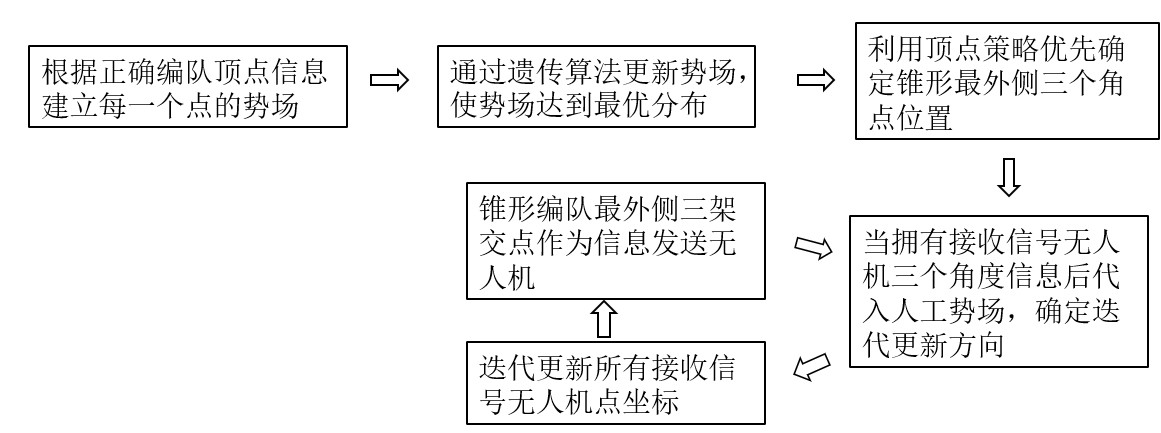
\includegraphics[width=1\textwidth]{wentisi.jpg}
    \caption{锥形无人机编队调整迭代过程图}
    \label{wentisi}
\end{figure}

由图\ref{wentisi}可知,延续模型三中建立正确点位置势场的想法,建立编队正确位置的优化人工势场模型。由于锥形图形没有圆形图形一样每一条通过圆心的直线都是对称轴的性质,因此当接收信息的无人机位置有较大偏离时,势场的中心往往不是无人机位置迭代更新的最优解。因此,我们需要对此情况进行特殊处理。本文提出利用遗传算法优化来初始化势场,以保证势场中的矢量指向达到最优分布,提高了模型的收敛性的同时也减小了模型的最终误差。

而对于锥形中发射信号无人机选择的问题,本文提出顶点策略的想法,\\

\textbf{第一部分:顶点策略}

由于锥形最外层角点离其它点距离较远,是无人机点集的一个凸包, 因此更适合作为发射信息的点。从由顶点向其它点修正信息,首先要保证顶点的位置相对准确。我们让顶点依次发送信息,这样每个顶点能获得其余两个点的方向。我们只需根据两个点的夹角,如果夹角比60度大,则前进,否则后退。
$$
\begin{cases}
        \alpha_1<60° , \textbf{无人机沿着}\alpha_1\textbf{角平分线且使}\alpha_1\textbf{角变大的方向运动}\\
        \alpha_1=60° , \textbf{无人机在瞬时时刻不运动}  \\                           
        \alpha_1>60° , \textbf{无人机沿着}\alpha_1\textbf{角平分线且使}\alpha_1\textbf{角变小的方向运动}\\
    \end{cases}
$$

借鉴上一问的思路,模拟其余两个顶点位置准确切此顶点的移动方向为两发射源的平均方向,计算不同位置该点所需移动的距离和夹角大小的关系,采用一维线性插值获得移动距离和夹角的方程即可。根据我们的测试,这种方法能让顶点收敛到$1e-16$的精度。

在校准顶点后,每个点都可根据顶点的角度信息进行调整。同样建立人工势场。我们只需要对边上的2种点,内部的一种点建立势场模型。\\

\textbf{第二部分:利用遗传算法自适应更新势场分布}

模型三中建立的势场的迭代更新向量均指向与正确编队位置的圆心处,但是若在锥形编队中无人机偏离正确位置过远时,仅基于优化人工势场的进行迭代向量更新时,会产生一部分不可继续优化的误差,因此我们想利用遗传优化算法来更改势场中固定向量的指向。优化其指向使其不再指向正确位置圆心处,而是指向经过遗传算法训练后迭代更新正确概率最大的一点。

遗传算法的训练步骤如下所示:

$1、$   固定人工选取的模拟势场的点位置不变,将每个点的势场强度向量代入遗传算法迭代,作为初始种群

$2、$   进化过程分为遗传和变异。选择若干向量更改之,即为变异。选择某点的向量设为种群中其它个体此位点的向量,即为遗传。将根据上一代信息获得遗传变异后的个体加入种群。

$3、$ 选取loss函数为各点临边(共30条)的累积误差作为目标函数,每次随机偏移每个飞行器位置作为训练数据,根据每个个体的势场迭代更新30此后计算loss

$4、$ 选取新种群目标函数前50\%小的个体作为新种群

$5、$ 重复上述 $2、3、4$ 步骤,待loss基本收敛

$6、$ 将结果输出


\subsubsection{模型的求解}

我们利用python程序(位于附录problem4.py中)在平面上依据正确图形随机生成变化范围在指定区间内的随机模型。

首先我们在正确的编队位置依据5.3中的人工势场模型建立势场。其次我们利用经过训练的遗传算法自适应势场分布,改变势场中迭代更新的向量方向与向量值,使之分布能使最终结果最优。

其次我们利用顶点策略更新锥形最外侧的三个点,使之能够利用相互之间的角度信息更新自身位置。在顶点更新到位后,转变为信号发射无人机。其余锥形边上点与锥形中的点作为信息接收点,通过正确编队中的势场确定迭代更新变量,从而实现逐步迭代更新,直至到达最优位置。

利用程序模拟锥形无人机编队调整与定位情况如图\ref{moxing4}所示:

\begin{figure}[h]
    \centering
    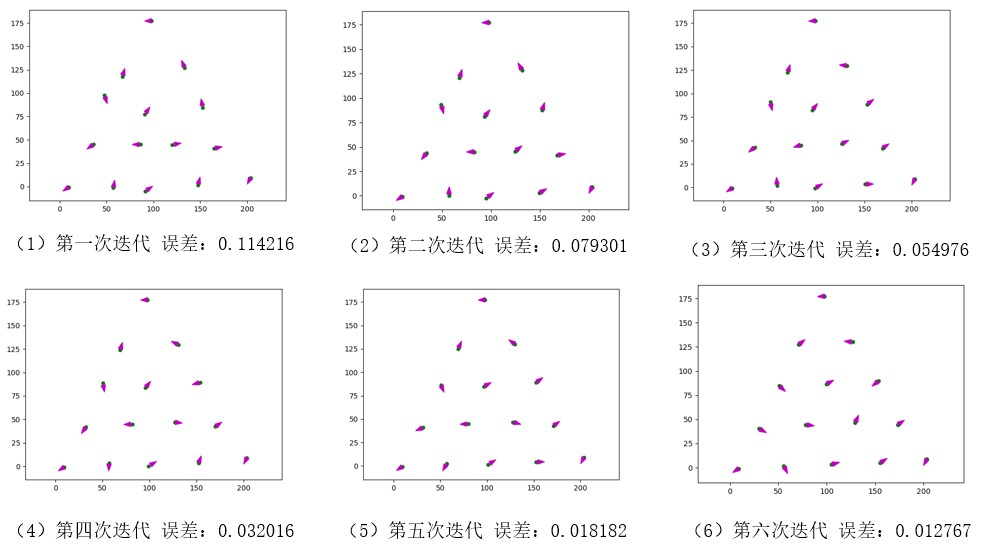
\includegraphics[width=1\textwidth]{moxing4.jpg}
    \caption{锥形无人机编队调整迭代过程图}
    \label{moxing4}
\end{figure}

从图\ref{moxing4}中也可以看出:利用本模型进行迭代更新,在6次迭代过后能够将原始误差下降10倍,到达0.012767的误差率。





%----------- 六、模型的分析与检验 ----------
\section{六、模型的分析与检验}

本文对问题三所构建的调整模型进行模型灵敏度分析。由问题三的分析可知,无人机初始点位置偏离正确位置的大小会对误差造成影响。因此我们通过对初始位置偏移最大值进行设定,在偏移最大值范围内产生测试点数据,将测试点数据代入模型三中进行求解。我们设定最大误差在1m-10m的范围之内,对范围内的测试点测试,并读取最终稳定误差值。

\begin{figure}[h]
    \centering
    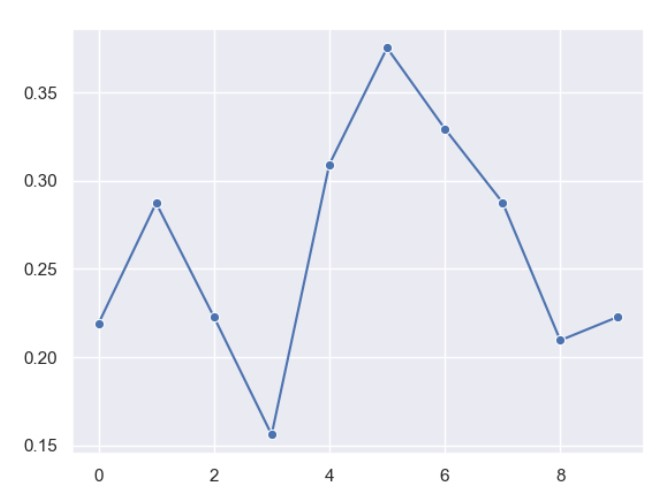
\includegraphics[width=0.5\textwidth]{mingandu.jpg}
    \caption{敏感度分析图}
    \label{lingmindu}
\end{figure}

如图\ref{lingmindu},调整后无人机编队的误差在0.15到0.37m之间波动,波动范围较小。在合理范围内增加产生点的位置偏差,模型所产生的误差在较小范围内波动,说明问题三所构建的模型稳定。




\section{七、模型的评价、改进与推广}


\subsection{模型的优点}
1. 在无人机距离目标越远时,调整的步长越大,因此在只有少数迭代次数的情况下就能快速收敛。

2. 本模型创新性的使用点云和KD树进行线性插值,使计算量大大降低。

3. 本模型的泛化性较强,可以用于不同形状的编队,而且只需要少数几个无人机发射信息即可做到所有无人机的调整。

4. 在手动建立的势场表现不好时还可使用遗传算法对势场做进一步优化。

\subsection{模型的缺点}
1. 本模型尚未对建立势场的选点调参,也未对遗传算法做响应调整。

2. 对于信息源的选取,也未探寻更优的策略。

3. 对于角度特征的映射只进行了简单的放射变换,角度特征在变换后的差异不够明显,导致选取临近点仍有误差。


\subsection{模型的拓展与推广}
1. 可以进一步探究发射无人机的选取和势场中预先选取点的指定,使调整精度更高。

2. 对于角度特征在空间中的映射,在不惜牺牲计算量的情况下可以使用更复杂的映射,甚至使用神经网络进行映射,使特征空间差异更加明显,更易进行向量检索,进一步提高精度。

3. 还可以使用强化学习更新势场,加速势场的训练。

\subsection{模型泛化性}
本文中仅把旋转对称的图形和规则多边形编队做为研究对象. 事实上, 对于不规则的编队仍能提供解决方案. 对于一个不规则编队, 可以计算凸包作为顶点, 顶点之间通过分组建立顶点策略, 再以顶点为信息源建立每一个内点的势场. 在做调整时先通过顶点策略确定顶点微调步长, 向信息源构成三角形的外心方向进行微调. 随后顶点作为信息源向其余内点发送角度信息, 让内点在提前建立好的势场中进行调整. 循环此过程即可.

%----------- 参考文献 ----------
\bibliographystyle{unsrt} %规定了参考文献的格式
\begin{center}
    \bibliography{reference} %调出LaTeX生成参考文献列表
\end{center}


\newpage
%----------- 附录 ----------
\newpage
\section{附录}

\begin{table}[htbp]
    \centering
    \begin{tabular}{|p{14.0cm}|}
 %指定单元格宽度, 并且水平居中。
    \hline
    \textbf{附件清单} \\ %换行 
    \hline
    1. 问题一主程序: \quad problem1.py \quad 用于问题一的坐标解算与做图分析 \\ 
    2. 问题二主程序:  \quad problem2.py \quad  用于问题二验证坐标信息并做图分析\\
    3. 问题三主程序:  \quad problem3.py \quad 用于问题三调整策略与调整策略展示\\
    4. 问题四主程序:  \quad problem4.py \quad 用于问题四调整策略加遗传算法计算\\
    \hline
    \end{tabular}
\end{table}

\lstinputlisting[
    style       =   Python,
    caption     =   {\bf problem1.py 用于解决问题一中坐标解算与做图},
    label       =   {problem1}
]{./problem1.py}

\lstinputlisting[
    style       =   Python,
    caption     =   {problem2.py 用于问题二中遍历算法与做图},
    label       =   {problem2.py}
]{./problem2.py}

\lstinputlisting[
    style       =   Python,
    caption     =   {problem3.py 用于问题三中迭代算法求解},
    label       =   {problem3.py}
]{./problem3.py}

\lstinputlisting[
    style       =   Python,
    caption     =   {problem4.py 用于问题四调整策略加遗传算法计算},
    label       =   {problem4.py}
]{./problem4.py}

\end{document}